\documentclass{standalone}
\usepackage{tikz}
\usetikzlibrary{patterns, positioning}


\begin{document}
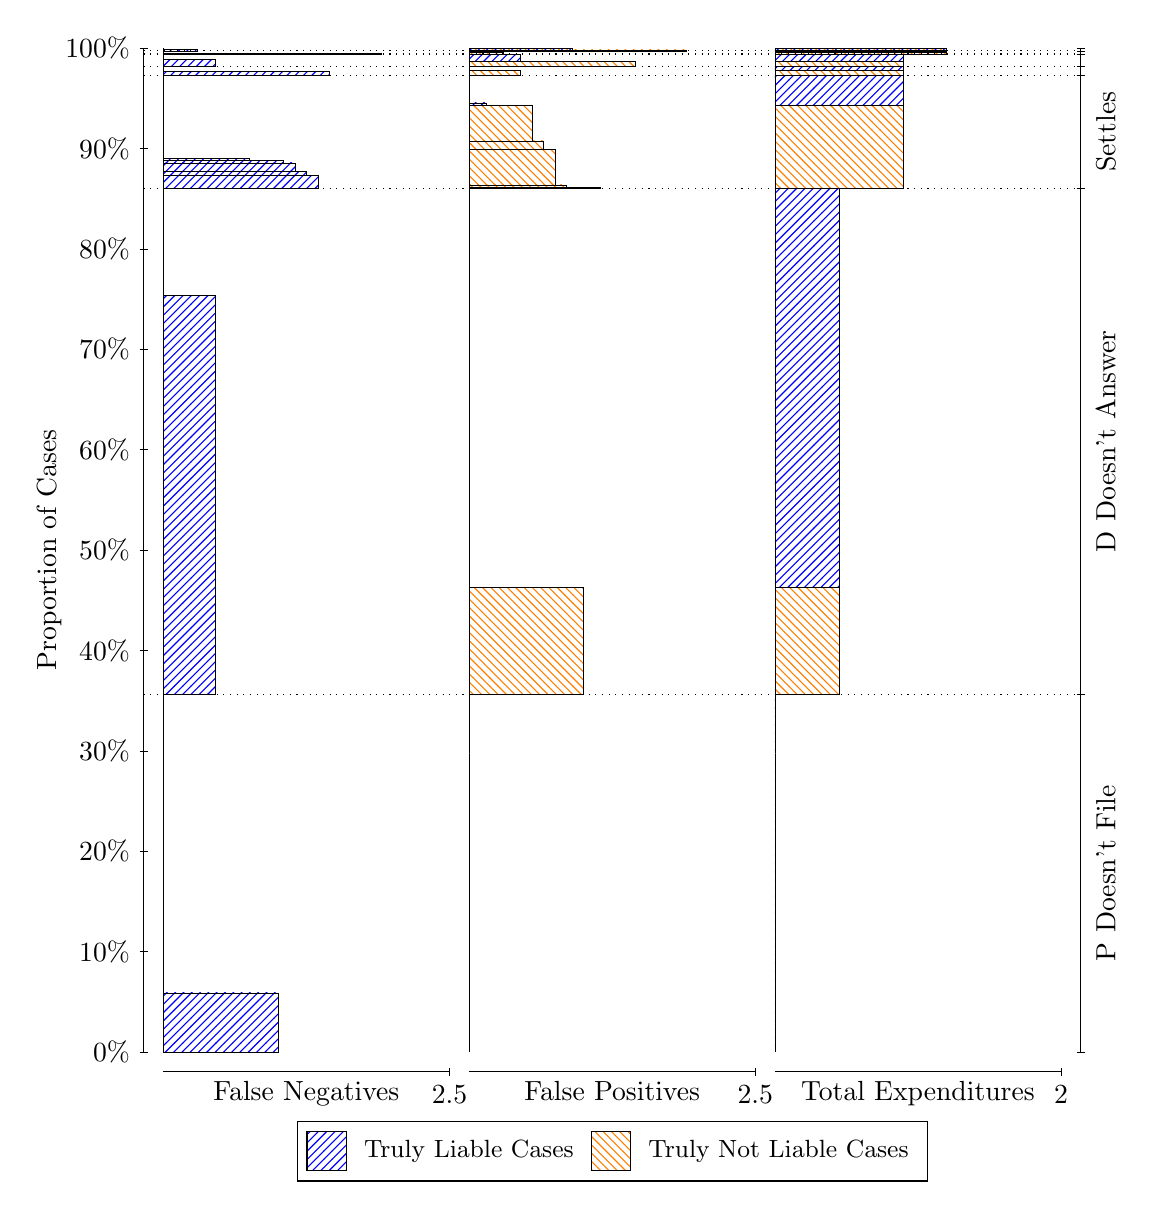
\begin{tikzpicture}
\draw[black, very thin] (1.5,1.75) -- (1.5,14.5);
\node[rotate=90, text=black, anchor=center] at (0.3, 8.125) {Proportion of Cases};
\draw[black, very thin] (1.45,1.75) -- (1.55,1.75);
\node[text=black, anchor=east] at (1.45, 1.75) {0\%};
\draw[black, very thin] (1.45,3.025) -- (1.55,3.025);
\node[text=black, anchor=east] at (1.45, 3.025) {10\%};
\draw[black, very thin] (1.45,4.3) -- (1.55,4.3);
\node[text=black, anchor=east] at (1.45, 4.3) {20\%};
\draw[black, very thin] (1.45,5.575) -- (1.55,5.575);
\node[text=black, anchor=east] at (1.45, 5.575) {30\%};
\draw[black, very thin] (1.45,6.85) -- (1.55,6.85);
\node[text=black, anchor=east] at (1.45, 6.85) {40\%};
\draw[black, very thin] (1.45,8.125) -- (1.55,8.125);
\node[text=black, anchor=east] at (1.45, 8.125) {50\%};
\draw[black, very thin] (1.45,9.4) -- (1.55,9.4);
\node[text=black, anchor=east] at (1.45, 9.4) {60\%};
\draw[black, very thin] (1.45,10.675) -- (1.55,10.675);
\node[text=black, anchor=east] at (1.45, 10.675) {70\%};
\draw[black, very thin] (1.45,11.95) -- (1.55,11.95);
\node[text=black, anchor=east] at (1.45, 11.95) {80\%};
\draw[black, very thin] (1.45,13.225) -- (1.55,13.225);
\node[text=black, anchor=east] at (1.45, 13.225) {90\%};
\draw[black, very thin] (1.45,14.5) -- (1.55,14.5);
\node[text=black, anchor=east] at (1.45, 14.5) {100\%};

\draw[black, very thin] (13.4,1.75) -- (13.4,14.5);
\draw[black, very thin] (13.35,1.75) -- (13.45,1.75);
\node[anchor=west] at (13.35, 1.75) {};
\draw[black, very thin] (13.35,6.293) -- (13.45,6.293);
\node[anchor=west] at (13.35, 6.293) {};
\draw[black, very thin] (13.35,12.721) -- (13.45,12.721);
\node[anchor=west] at (13.35, 12.721) {};
\draw[black, very thin] (13.35,14.153) -- (13.45,14.153);
\node[anchor=west] at (13.35, 14.153) {};
\draw[black, very thin] (13.35,14.262) -- (13.45,14.262);
\node[anchor=west] at (13.35, 14.262) {};
\draw[black, very thin] (13.35,14.424) -- (13.45,14.424);
\node[anchor=west] at (13.35, 14.424) {};
\draw[black, very thin] (13.35,14.463) -- (13.45,14.463);
\node[anchor=west] at (13.35, 14.463) {};
\draw[black, very thin] (13.35,14.5) -- (13.45,14.5);
\node[anchor=west] at (13.35, 14.5) {};

\draw[black, very thin, pattern color=blue, pattern=north east lines] (1.75,1.75) rectangle (3.2033,2.5016);
\draw[black, very thin, pattern color=orange, pattern=north west lines] (1.75,2.5016) rectangle (1.75,6.293);
\draw[black, very thin, pattern color=blue, pattern=north east lines] (1.75,6.293) rectangle (2.404,11.363);
\draw[black, very thin, pattern color=orange, pattern=north west lines] (1.75,11.363) rectangle (1.75,12.721);
\draw[black, very thin, pattern color=blue, pattern=north east lines] (1.75,12.721) rectangle (3.712,12.882);
\draw[black, very thin, pattern color=blue, pattern=north east lines] (1.75,12.882) rectangle (3.5667,12.93);
\draw[black, very thin, pattern color=blue, pattern=north east lines] (1.75,12.93) rectangle (3.4213,13.04);
\draw[black, very thin, pattern color=blue, pattern=north east lines] (1.75,13.04) rectangle (3.276,13.069);
\draw[black, very thin, pattern color=blue, pattern=north east lines] (1.75,13.069) rectangle (3.1307,13.07);
\draw[black, very thin, pattern color=blue, pattern=north east lines] (1.75,13.07) rectangle (2.84,13.099);
\draw[black, very thin, pattern color=orange, pattern=north west lines] (1.75,13.099) rectangle (1.75,14.153);
\draw[black, very thin, pattern color=blue, pattern=north east lines] (1.75,14.153) rectangle (3.8573,14.199);
\draw[black, very thin, pattern color=orange, pattern=north west lines] (1.75,14.199) rectangle (1.75,14.262);
\draw[black, very thin, pattern color=blue, pattern=north east lines] (1.75,14.262) rectangle (2.404,14.354);
\draw[black, very thin, pattern color=orange, pattern=north west lines] (1.75,14.354) rectangle (1.75,14.424);
\draw[black, very thin, pattern color=blue, pattern=north east lines] (1.75,14.424) rectangle (4.5113,14.436);
\draw[black, very thin, pattern color=orange, pattern=north west lines] (1.75,14.436) rectangle (1.75,14.463);
\draw[black, very thin, pattern color=blue, pattern=north east lines] (1.75,14.463) rectangle (2.186,14.487);
\draw[black, very thin, pattern color=orange, pattern=north west lines] (1.75,14.487) rectangle (1.75,14.5);
\draw[black, very thin, pattern color=orange, pattern=north west lines] (5.6333,1.75) rectangle (5.6333,5.5414);
\draw[black, very thin, pattern color=blue, pattern=north east lines] (5.6333,5.5414) rectangle (5.6333,6.293);
\draw[black, very thin, pattern color=orange, pattern=north west lines] (5.6333,6.293) rectangle (7.0867,7.6509);
\draw[black, very thin, pattern color=blue, pattern=north east lines] (5.6333,7.6509) rectangle (5.6333,12.721);
\draw[black, very thin, pattern color=orange, pattern=north west lines] (5.6333,12.721) rectangle (7.3047,12.731);
\draw[black, very thin, pattern color=orange, pattern=north west lines] (5.6333,12.731) rectangle (7.014,12.732);
\draw[black, very thin, pattern color=orange, pattern=north west lines] (5.6333,12.732) rectangle (6.8687,12.762);
\draw[black, very thin, pattern color=orange, pattern=north west lines] (5.6333,12.762) rectangle (6.7233,13.217);
\draw[black, very thin, pattern color=orange, pattern=north west lines] (5.6333,13.217) rectangle (6.578,13.321);
\draw[black, very thin, pattern color=orange, pattern=north west lines] (5.6333,13.321) rectangle (6.4327,13.774);
\draw[black, very thin, pattern color=blue, pattern=north east lines] (5.6333,13.774) rectangle (5.8513,13.804);
\draw[black, very thin, pattern color=blue, pattern=north east lines] (5.6333,13.804) rectangle (5.6333,14.153);
\draw[black, very thin, pattern color=orange, pattern=north west lines] (5.6333,14.153) rectangle (6.2873,14.215);
\draw[black, very thin, pattern color=blue, pattern=north east lines] (5.6333,14.215) rectangle (5.6333,14.262);
\draw[black, very thin, pattern color=orange, pattern=north west lines] (5.6333,14.262) rectangle (7.7407,14.331);
\draw[black, very thin, pattern color=blue, pattern=north east lines] (5.6333,14.331) rectangle (6.2873,14.424);
\draw[black, very thin, pattern color=orange, pattern=north west lines] (5.6333,14.424) rectangle (6.0693,14.45);
\draw[black, very thin, pattern color=blue, pattern=north east lines] (5.6333,14.45) rectangle (5.6333,14.463);
\draw[black, very thin, pattern color=orange, pattern=north west lines] (5.6333,14.463) rectangle (8.3947,14.476);
\draw[black, very thin, pattern color=blue, pattern=north east lines] (5.6333,14.476) rectangle (6.9413,14.5);
\draw[black, very thin, pattern color=orange, pattern=north west lines] (9.5167,1.75) rectangle (9.5167,5.5414);
\draw[black, very thin, pattern color=blue, pattern=north east lines] (9.5167,5.5414) rectangle (9.5167,6.293);
\draw[black, very thin, pattern color=orange, pattern=north west lines] (9.5167,6.293) rectangle (10.334,7.6509);
\draw[black, very thin, pattern color=blue, pattern=north east lines] (9.5167,7.6509) rectangle (10.334,12.721);
\draw[black, very thin, pattern color=orange, pattern=north west lines] (9.5167,12.721) rectangle (11.152,13.774);
\draw[black, very thin, pattern color=blue, pattern=north east lines] (9.5167,13.774) rectangle (11.152,14.153);
\draw[black, very thin, pattern color=orange, pattern=north west lines] (9.5167,14.153) rectangle (11.152,14.215);
\draw[black, very thin, pattern color=blue, pattern=north east lines] (9.5167,14.215) rectangle (11.152,14.262);
\draw[black, very thin, pattern color=orange, pattern=north west lines] (9.5167,14.262) rectangle (11.152,14.331);
\draw[black, very thin, pattern color=blue, pattern=north east lines] (9.5167,14.331) rectangle (11.152,14.424);
\draw[black, very thin, pattern color=orange, pattern=north west lines] (9.5167,14.424) rectangle (11.697,14.45);
\draw[black, very thin, pattern color=blue, pattern=north east lines] (9.5167,14.45) rectangle (11.697,14.463);
\draw[black, very thin, pattern color=orange, pattern=north west lines] (9.5167,14.463) rectangle (11.697,14.476);
\draw[black, very thin, pattern color=blue, pattern=north east lines] (9.5167,14.476) rectangle (11.697,14.5);
\draw[black, dotted] (1.5,6.293) -- (13.4,6.293);
\draw[black, dotted] (1.5,12.721) -- (13.4,12.721);
\draw[black, dotted] (1.5,14.153) -- (13.4,14.153);
\draw[black, dotted] (1.5,14.262) -- (13.4,14.262);
\draw[black, dotted] (1.5,14.424) -- (13.4,14.424);
\draw[black, dotted] (1.5,14.463) -- (13.4,14.463);
\draw[black, very thin] (1.75,1.5) -- (5.3833,1.5);
\node[text=black, anchor=north] at (3.5667, 1.5) {False Negatives};
\draw[black, very thin] (5.3833,1.45) -- (5.3833,1.55);
\node[text=black, anchor=north] at (5.3833, 1.45) {2.5};

\draw[black, very thin] (5.6333,1.5) -- (9.2667,1.5);
\node[text=black, anchor=north] at (7.45, 1.5) {False Positives};
\draw[black, very thin] (9.2667,1.45) -- (9.2667,1.55);
\node[text=black, anchor=north] at (9.2667, 1.45) {2.5};

\draw[black, very thin] (9.5167,1.5) -- (13.15,1.5);
\node[text=black, anchor=north] at (11.333, 1.5) {Total Expenditures};
\draw[black, very thin] (13.15,1.45) -- (13.15,1.55);
\node[text=black, anchor=north] at (13.15, 1.45) {2};

\node[text=black, centered, rotate=90] at (13.72, 4.0215) {P Doesn't File};
\node[text=black, centered, rotate=90] at (13.72, 9.5068) {D Doesn't Answer};
\node[text=black, centered, rotate=90] at (13.72, 13.437) {Settles};





\draw (7.449999999999999,1.5) node[draw=none] (baseCoordinate) {};
\begin{scope}[align=center]
        \matrix[scale=0.5, draw=black, below=0.5cm of baseCoordinate, nodes={draw}, column sep=0.1cm]{
            \node[rectangle, draw, minimum width=0.5cm, minimum height=0.5cm, pattern color=blue, pattern=north east lines] {}; &
            \node[draw=none, font=\small, text=black] (B) {Truly Liable Cases}; &
            \node[rectangle, draw, minimum width=0.5cm, minimum height=0.5cm, pattern color=orange, pattern=north west lines] {}; &
            \node[draw=none, font=\small, text=black] (B) {Truly Not Liable Cases}; \\
            };
\end{scope}

\end{tikzpicture}
\end{document}